The Table \ref{tab:bpm_table_blind} presents the average heart rate by each blind participant on each scenes. It is possible to see that the previous expectation cannot be proven, since there is no sistematic pattern in the heartrate variation between the rounds.


\begin{table}[!htb]
\centering
\caption{Average BPM felled by the blinded participants [BPM].}
\label{tab:bpm_table_blind}
\begin{tabular}{llrrrrr}
\toprule
     &        &   Base &  Audio & \begin{tabular}[c]{@{}l@{}}Haptic\\ Belt\end{tabular} & \begin{tabular}[c]{@{}l@{}}Virtual\\ Cane\end{tabular} & Mixture \\
Participant & Round &        &        &                                                       &                                                        &         \\
\midrule
001C & First &  75.75 &  60.71 &                                                 71.17 &                                                  59.07 &   68.24 \\
     & Return &  71.05 &  58.61 &                                                 66.22 &                                                  64.20 &   70.76 \\
002C & First &  48.69 &  38.67 &                                                 48.74 &                                                  46.89 &   52.23 \\
     & Return &  52.46 &  47.58 &                                                 58.97 &                                                  56.75 &   58.25 \\
003C & First &  68.37 &  69.89 &                                                 70.95 &                                                  69.41 &   66.94 \\
     & Return &  67.34 &  67.44 &                                                 69.68 &                                                  68.82 &   67.37 \\
004C & First &  75.09 &  73.55 &                                                 73.70 &                                                  71.94 &   74.03 \\
     & Return &  74.74 &  74.79 &                                                 74.02 &                                                  72.69 &   67.34 \\
\bottomrule
\end{tabular}
\end{table}



In the Figure \ref{fig:barplot_ecg_bpm_5_scene_blind} is plotted the average data presentend in the previoes table. There is a slight increase in the heartrate between the rounds, with the exception of the "Base" method. That means that, in the average, the participants felt more demandful in the "Return" round.

\begin{figure}[!htb]
    \centering
    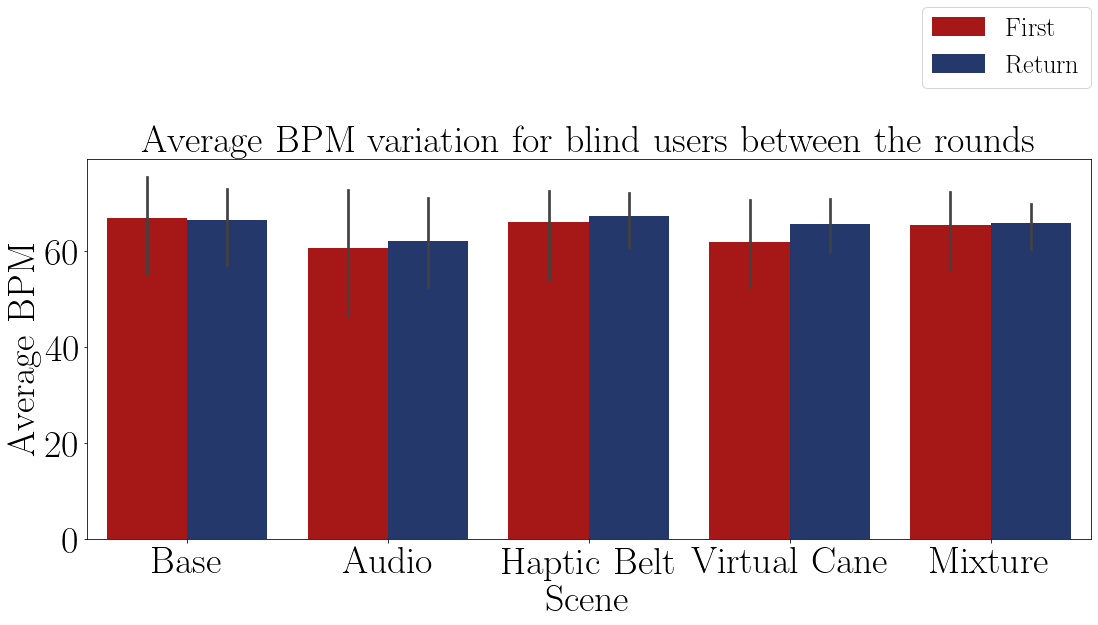
\includegraphics[width = 0.8\linewidth]{Resultados/ECG/Figuras/png/barplot_ecg_bpm_5_scene_blind.png}
    \caption{Barplot of the average BPM of the blind participants on each method.}
    \label{fig:barplot_ecg_bpm_5_scene_blind}
\end{figure}

The Table \ref{tab:bpm_average_group_blind} show the average heartbeat frequency variation between the rounds of each group. As it was shown in the Figure \ref{fig:barplot_ecg_bpm_5_scene_blind}, only the "Base" method has a negative average variaton between the rounds. It is also posible to see that the Virtual Cane variation was the highest, hence it was also the highest mental workload.
 

\begin{table}[!htb]
\centering
\caption{ECG average BPM  for each method of the blind participants.}
\label{tab:bpm_average_group_blind}
\begin{tabular}{lrrrrr}
\toprule
{} &   Base & Audio & Haptic Belt & Virtual Cane & Mixture \\
Visual Condition &        &       &             &              &         \\
\midrule
Blind            &  -0.58 &  1.40 &        1.09 &         3.79 &    0.57 \\
\bottomrule
\end{tabular}
\end{table}



The Figure \ref{fig:boxplot_ecg_bpm_blind_scene} show a comparison between the methods. There is no big difference between them, but it is posible to 
separate them in two groups based on their similarity. One with “Base”, “Haptic Belt” and “Mixture” methods and the other with “Audio” and “Virtual Cane”. The Figure \ref{fig:boxplot_ecg_bpm_blind_rounds} presents the average heartreate frequency grouped by round.

\begin{figure}[!htb]
    \centering
    \begin{minipage}{0.45\textwidth}
        \centering
        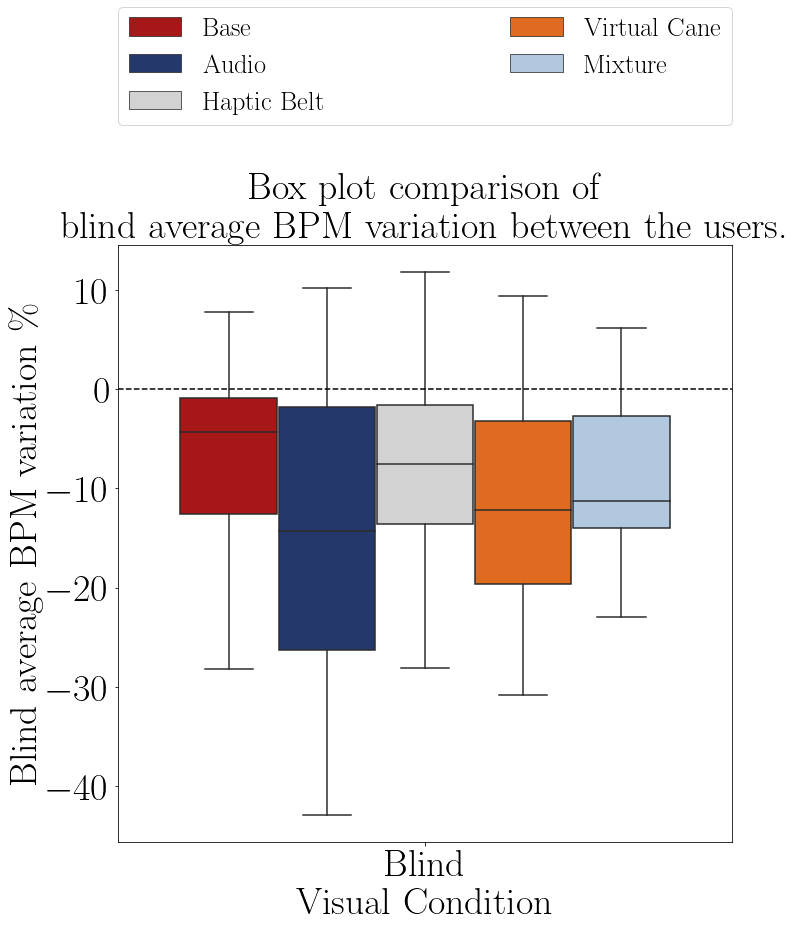
\includegraphics[width = 0.8\linewidth]{Resultados/ECG/Figuras/png/boxplot_ecg_bpm_blind_scene.png}
        \caption{Boxplot of the BPM of the blind participants grouped by method.}
        \label{fig:boxplot_ecg_bpm_blind_scene}
    \end{minipage}
    \begin{minipage}{0.45\textwidth}
        \centering
        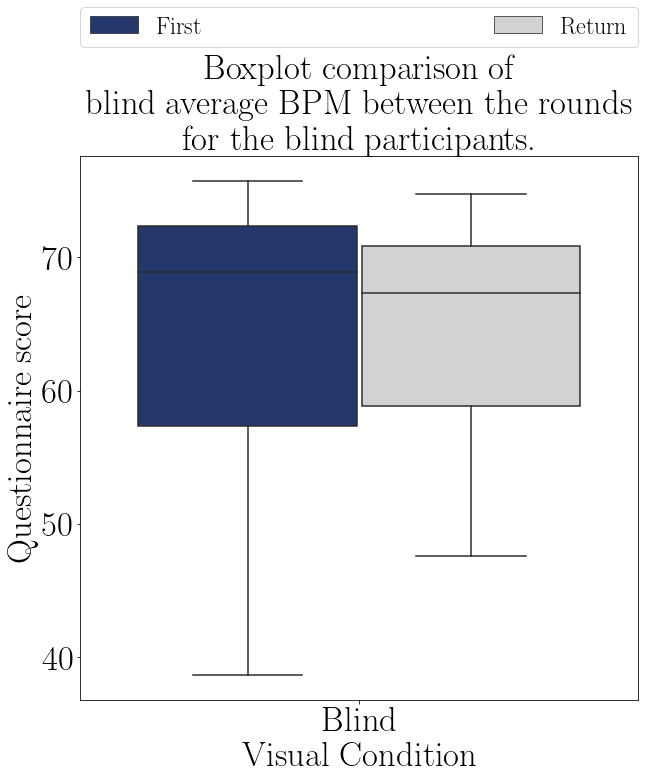
\includegraphics[width = 0.8\linewidth]{Resultados/ECG/Figuras/png/boxplot_ecg_bpm_blind_rounds.png}
        \caption{Boxplot of the BPM of the blind participants grouped by round.}
        \label{fig:boxplot_ecg_bpm_blind_rounds}
    \end{minipage}
\end{figure}

The Figures \ref{fig:qqplot_bpm_two_way} and \ref{fig:residplot_bpm_two_way} shows the distribution and variance of the Table \ref{tab:bpm_table_blind}. These Figures shows that the data are normally distributed but the participants had different  that the methods have a similar variance.
The Table \ref{tab:blocanova_bpm_two_way} shows the ANOVA test p-value of the heart rate frequency of the “blind” sample. The p-value indicates that there is no effect of the methods, rounds and neither their interaction in the heartrate frequency.


\begin{table}[!htb]
\centering
\caption{Anova p-value for the BPM on each method for blinded users.}
\label{tab:blocanova_bpm_two_way}
\begin{tabular}{lrrrrr}
\toprule
               Source &  Squared sum &  DOF & Squared average &      F & \begin{tabular}[c]{@{}l@{}}P-Value \\ $(F_{0} > F)$\end{tabular} \\
\midrule
Participants (Blocks) &     2807.274 &    3 &         935.758 & 49.361 &                                                                  \\
         \    Methods &      164.045 &    4 &          41.011 &  2.163 &                                                            0.100 \\
          \    Rounds &       15.693 &    1 &          15.693 &  0.828 &                                                            0.371 \\
     \    Interaction &       20.606 &    4 &           5.152 &  0.272 &                                                            0.894 \\
   Experimental Error &      511.853 &   27 &          18.958 &        &                                                                  \\
                Total &     3519.471 &   39 &                 &        &                                                                  \\
\bottomrule
\end{tabular}
\end{table}



\begin{figure}[!htb]
    \centering
    \begin{minipage}{0.45\textwidth}
        \centering
        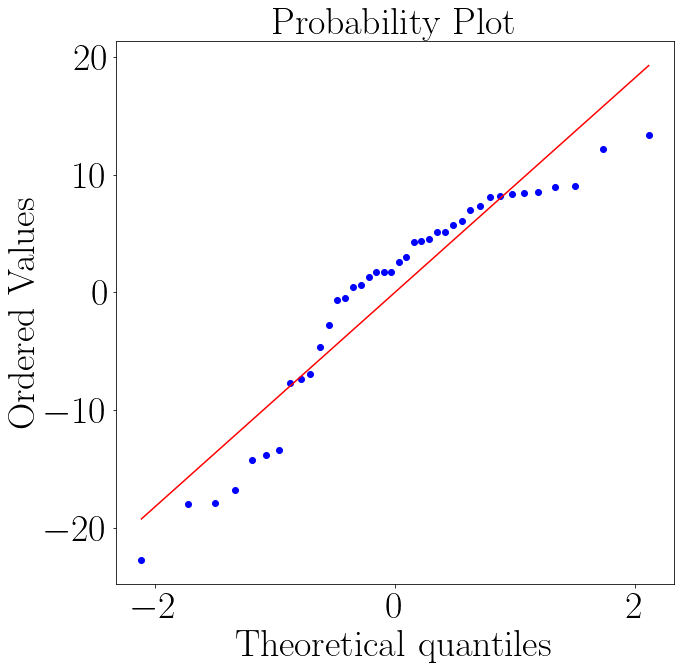
\includegraphics[width = 0.8\linewidth]{Resultados/ECG/Figuras/png/qqplot_bpm_two_way.png}
        \caption{QQ plot of the BPM of the blind participants on each method.}
        \label{fig:qqplot_bpm_two_way}
    \end{minipage}
    \begin{minipage}{0.45\textwidth}
        \centering
        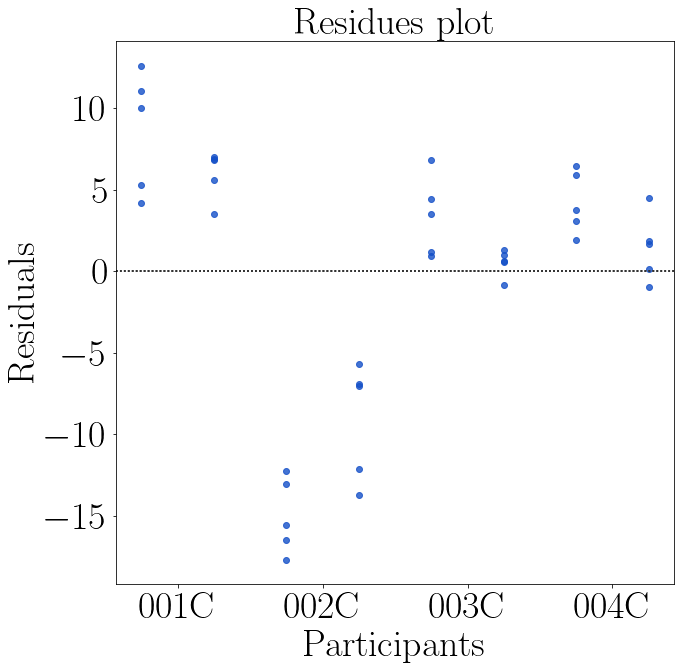
\includegraphics[width = 0.8\linewidth]{Resultados/ECG/Figuras/png/residplot_bpm_two_way.png}
        \caption{Residual plot of the BPM score the blind participants on each method.}
        \label{fig:residplot_bpm_two_way}
    \end{minipage}
\end{figure}


%
\begin{table}[!htb]
\centering
\caption{Cross validation p-value for the average BPM on each method for blinded users.}
\label{tab:lsd_bpm_two_way}
\begin{tabular}{rclr}
\toprule
      \multicolumn{3}{c}{Method} &                                           Analysis \\
\midrule
              Base & $X$ & Audio &               $H_1 : \mu_{Base} \ne \mu_{Audio}**$ \\
        Base & $X$ & Haptic Belt &             $H_0 : \mu_{Base} = \mu_{Haptic Belt}$ \\
       Base & $X$ & Virtual Cane &        $H_1 : \mu_{Base} \ne \mu_{Virtual Cane}**$ \\
            Base & $X$ & Mixture &             $H_1 : \mu_{Base} \ne \mu_{Mixture}**$ \\
       Audio & $X$ & Haptic Belt &        $H_1 : \mu_{Audio} \ne \mu_{Haptic Belt}**$ \\
      Audio & $X$ & Virtual Cane &       $H_1 : \mu_{Audio} \ne \mu_{Virtual Cane}**$ \\
           Audio & $X$ & Mixture &            $H_1 : \mu_{Audio} \ne \mu_{Mixture}**$ \\
Haptic Belt & $X$ & Virtual Cane & $H_1 : \mu_{Haptic Belt} \ne \mu_{Virtual Cane}**$ \\
     Haptic Belt & $X$ & Mixture &      $H_1 : \mu_{Haptic Belt} \ne \mu_{Mixture}**$ \\
    Virtual Cane & $X$ & Mixture &     $H_1 : \mu_{Virtual Cane} \ne \mu_{Mixture}**$ \\
\bottomrule
\end{tabular}
\end{table}



%The Table \ref{tab:lsd_bpm_two_way} presents the conclusion of a pairwise Fisher LSD test of the blind heart rate frequency variation between all the guidance methods. The results show that the only the "Base" and "Haptic belt" have simila reaction.

According to the ANOVA test at Table \ref{tab:blocanova_bpm_two_way}, there is no effect from the method, the round or the interaction between them in the heartrate frequency. It is posible to notice some small difference in the Figure \ref{fig:boxplot_ecg_bpm_blind_scene} but maybe because of the small sample size, it was no sensitive enough to be proved by the ANOVA test. But inside that Figure

\FloatBarrier